%%%%%%%% ICML 2025 EXAMPLE LATEX SUBMISSION FILE %%%%%%%%%%%%%%%%%

\documentclass{article}

% Recommended, but optional, packages for figures and better typesetting:
\usepackage{microtype}
\usepackage{graphicx}
\usepackage{subfigure}
\usepackage{booktabs} % for professional tables

% hyperref makes hyperlinks in the resulting PDF.
% If your build breaks (sometimes temporarily if a hyperlink spans a page)
% please comment out the following usepackage line and replace
% \usepackage{icml2025} with \usepackage[nohyperref]{icml2025} above.
\usepackage{hyperref}


% Attempt to make hyperref and algorithmic work together better:
\newcommand{\theHalgorithm}{\arabic{algorithm}}

% Use the following line for the initial blind version submitted for review:
\usepackage[accepted]{icml2025}

% If accepted, instead use the following line for the camera-ready submission:
% \usepackage[accepted]{icml2025}

% For theorems and such
\usepackage{amsmath}
\usepackage{amssymb}
\usepackage{mathtools}
\usepackage{amsthm}

% if you use cleveref..
\usepackage[capitalize,noabbrev]{cleveref}

%%%%%%%%%%%%%%%%%%%%%%%%%%%%%%%%
% THEOREMS
%%%%%%%%%%%%%%%%%%%%%%%%%%%%%%%%
\theoremstyle{plain}
\newtheorem{theorem}{Theorem}[section]
\newtheorem{proposition}[theorem]{Proposition}
\newtheorem{lemma}[theorem]{Lemma}
\newtheorem{corollary}[theorem]{Corollary}
\theoremstyle{definition}
\newtheorem{definition}[theorem]{Definition}
\newtheorem{assumption}[theorem]{Assumption}
\theoremstyle{remark}
\newtheorem{remark}[theorem]{Remark}

% Todonotes is useful during development; simply uncomment the next line
%    and comment out the line below the next line to turn off comments
%\usepackage[disable,textsize=tiny]{todonotes}
\usepackage[textsize=tiny]{todonotes}


% The \icmltitle you define below is probably too long as a header.
% Therefore, a short form for the running title is supplied here:
\icmltitlerunning{Large-Scale Procedural Robot Generation}

\begin{document}

\twocolumn[
\icmltitle{Large-Scale Procedural Robot Generation}

% It is OKAY to include author information, even for blind
% submissions: the style file will automatically remove it for you
% unless you've provided the [accepted] option to the icml2025
% package.

% List of affiliations: The first argument should be a (short)
% identifier you will use later to specify author affiliations
% Academic affiliations should list Department, University, City, Region, Country
% Industry affiliations should list Company, City, Region, Country

% You can specify symbols, otherwise they are numbered in order.
% Ideally, you should not use this facility. Affiliations will be numbered
% in order of appearance and this is the preferred way.
\icmlsetsymbol{equal}{*}

\begin{icmlauthorlist}
\icmlauthor{Nurhak Yalcin}{tud}
\icmlauthor{Lukas Müller}{tud}
\icmlauthor{Nico Bohlinger}{ias}
%\icmlauthor{}{sch}
%\icmlauthor{}{sch}
%\icmlauthor{}{sch}
\end{icmlauthorlist}

\icmlaffiliation{tud}{Department of Computer Science, Technische Universität Darmstadt, Germany}
\icmlaffiliation{ias}{Department of Computer Science, Intelligent Autonomous Systems Group, Technische Universität Darmstadt, Germany}

\icmlcorrespondingauthor{Nurhak Yalcin}{nurhak.yalcin@stud.tu-darmstadt.de}
\icmlcorrespondingauthor{Lukas Müller}{lukas.mueller1@stud.tu-darmstadt.de}
\icmlcorrespondingauthor{Nico Bohlinger}{nico.bohlinger@tu-darmstadt.de}

\vskip 0.3in
]

% this must go after the closing bracket ] following \twocolumn[ ...

% This command actually creates the footnote in the first column
% listing the affiliations and the copyright notice.
% The command takes one argument, which is text to display at the start of the footnote.
% The \icmlEqualContribution command is standard text for equal contribution.
% Remove it (just {}) if you do not need this facility.

\printAffiliationsAndNotice{}  % leave blank if no need to mention equal contribution

\begin{abstract}
We present a system for large-scale generation of diverse robot embodiments. Unlike existing approaches that rely on prior knowledge and thus limit the embodiment design space, our system leverages a Variational Autoencoder with a message-passing graph neural network that can be trained directly on existing robot designs. As the Variational Autoencoder learns a continuous latent space of morphologies, this approach potentially enables sampling thousands of valid, physically plausible designs. Experiments on synthetic datasets and real robot designs show that our system can reconstruct unseen robots and generate novel embodiments that are suitable for downstream tasks. This paves the way for both task-agnostic robot generation and morphology-agnostic policy learning.
\end{abstract}

\section{Introduction}
Foundational models in robot learning aim to generalize the capability to perform a given task, independent of robot embodiments, environment characteristics or task variations. Especially in locomotion, a foundational model needs to be agnostic of the specific robot design in order to be used for new and unseen robots. To achieve this generalization, a large number of diverse robots is needed as training examples. Recent work has shown that increasing the number of training embodiments improves the generalization to unseen ones \cite{ai2025towards}.

The design space of robot embodiments is large and grows exponentially with the number of components of the robot. Therefore, a systematic approach for exploring the numerous design options and based on this, procedurally generating new designs is needed. Existing automated approaches address this through grammar-based methods \cite{zhao2020robogrammar, hu2023glso}, which construct robots from a predefined library of body parts. These methods suffer from several drawbacks: they require prior knowledge to define the component library, restrict design to discrete combinations and produce robots that might not reflect the complexity of real-world systems with continuous physical parameters such as mass, friction, or stiffness.

In this work, we present an end-to-end system that approaches this problem by using a Variational Autoencoder (VAE), implemented by a Message Passing Graph Neural Network (MPNN). The VAE learns a latent space representation and a probability distribution of robots. 

The training examples consist of both the robot kinematic structures and the attributes of the body parts of each robot. Instead of predicting discrete components, our method regresses continuous feature values, capturing realistic properties like mass, geometry and joint specifications. This enables the generation of physically plausible designs that are closer to robots already used in research and industry.

\section{Related Work}
\subsection{Evolutionary Algorithms}
Evolutionary algorithms have been used for robot design automation, typically optimizing morphology and control simultaneously through population-based search methods. \citet{sims1994evolving} pioneered the co-evolution of morphology and control in simulated creatures, while more recent work by \citet{wangneural} introduced Neural Graph Evolution (NGE), which evolves robot structures over arbitrary graph topologies. 

These approaches rely on task-specific fitness functions to guide the evolutionary process, which require extensive computational resources as each robot morphology candidate must be evaluated through complete policy learning for specific tasks. This dependence on task-specific rewards limits the ability of discovered morphologies to generalize well, as the fitness landscape changes across different objectives.

\subsection{Cross-Embodiment Policy Learning}

A related line of work focuses on policies that generalize across robot morphologies. \citet{bohlinger2024one} introduced the Unified Robot Morphology Architecture (URMA),
an end-to-end reinforcement learning framework with morphology-agnostic encoders and decoders.
URMA was trained on 16 robots and learns a locomotion policy that is transferable to unseen robots in simulation and the real world. However, it remains limited to locomotion tasks.

This idea was extended by studying embodiment scaling laws \cite{ai2025towards}. Using
GENBOT-1K, a dataset of $\sim$1,000 procedurally generated robots, they showed that more diverse
training embodiments improve generalization and enable zero-shot transfer to real robots.

Motivated by this finding, our approach focuses on generating a large number of diverse robot embodiments that are independent of a specific objective. These robots can then be used for downstream tasks like locomotion and improve generalization abilities.

\subsection{Task-Agnostic Morphology Discovery}

Recent work has begun to explore the optimization of robot morphologies without explicit task specifications. Task-Agnostic Morphology Evolution (TAME) \cite{hejna2021task} represents this new approach by using information-theoretic objectives to evaluate morphologies without task-specific rewards. 

Their method uses mutual information between states and actions as an approximation for how effective a morphology is, capturing both its ability to explore and its controllability. This approach uses Entropy-based metrics to measure the diversity of the states a robot goes through and the predictability of these movements, which provides a statistical framework for morphology evaluation. 

This information-theoretic approach allows us to statistically differentiate between morphologies based on their general capabilities rather than on a specific task performance, which aligns well with our goal of developing a statistical view on robot populations.

\subsection{RoboGrammar and GLSO}

Graph grammar-based approaches have emerged as tools for constraining the morphological search space while maintaining design diversity. RoboGrammar \cite{zhao2020robogrammar} introduced recursive graph grammar rules to generate terrain-optimized robots, representing morphologies as directed acyclic graphs where vertices represent limbs and edges represent joints. 

This grammatical approach ensures physical feasibility while enabling systematic exploration of the design space. Building upon this foundation, Grammar-guided Latent Space Optimization (GLSO) \cite{hu2023glso} combines graph grammar rules with VAEs to learn continuous latent representations of discrete morphological designs. GLSO addresses the computational challenges of morphology-behavior optimization by transforming the discrete combinatorial optimization problem into a continuous one, where Bayesian Optimization can be applied efficiently. The VAE learns a mapping between graph-structured robot designs and a low-dimensional latent space, with training guided by both reconstruction objectives and robot world-space features. 

This approach enables the generation of large populations of morphologically diverse robots without having to evaluate specific tasks, as the latent space captures morphological similarity based on structural and physical properties and not on performance metrics.

\section{Preliminaries}
\subsection{Variational Autoencoder} \label{vae}
A VAE is a generative model that learns a probabilistic mapping between the input data and a latent space \cite{kingma2014auto}. The model consists of an encoder and decoder neural network. 

In the encoder, the input data $x$ is mapped to a latent distribution $q_\phi(z \mid x)$, which is typically a Gaussian parametrized by a mean $\mu$ and variance $\sigma^2$. The decoder network reconstructs the input from sampled latent variables $p_\theta(x \mid z)$. 

\begin{figure*}[t]
    \centering
    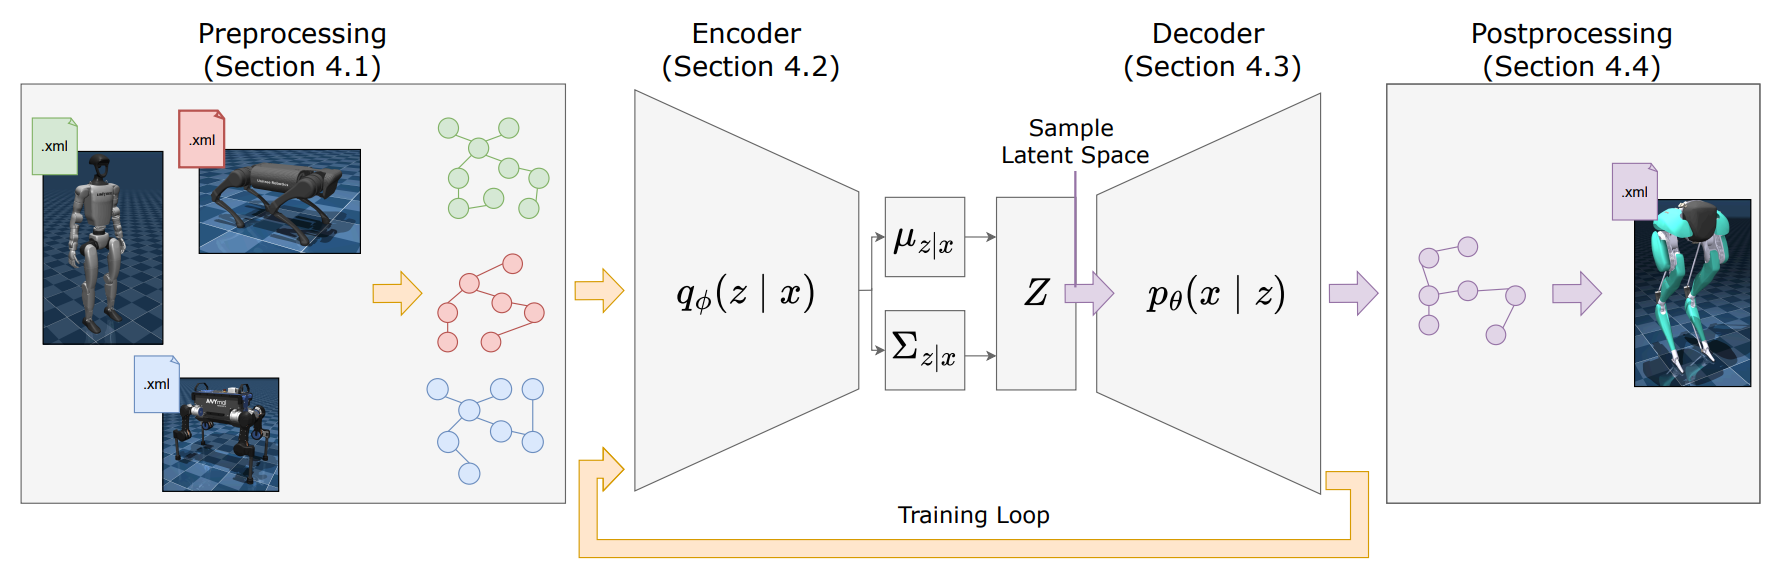
\includegraphics[width=\textwidth]{figures/lascroge_overview2.drawio.png}
    \caption{Overview of the end-to-end system, which consists of pre- and postprocessing, the encoder and the decoder. The orange arrows represent the training loop which consists of encoding the robot designs that serve as training data, computing the loss and performing backpropagation to update the learnable parts of the system. The purple arrows represents the process of generating new robots by sampling from the latent space, decoding the latent vector and postprocess to retrieve the .xml MuJoCo file.}
    \label{fig:overview}
\end{figure*}

During training, the VAE optimizes the Evidence Lower Bound (ELBO) which balances the reconstruction accuracy with a regularization term that enforces similarity between the learned latent distribution and a prior distribution. The standard choice for this prior is a multivariate Gaussian $p(z) = \mathcal{N}(0, \mathbf{I})$.

After training, new samples can be generated by sampling from the latent space $p(z)$ and passing these through the decoder. This probabilistic framework makes VAEs suitable to procedurally generate a large number of robot embodiments, based on the training examples that were provided. Consequently, we hypothesize that if the model is trained on a diverse set of embodiments it is easy to generate a large number of new robots by sampling from the latent space and using the decoder and the postprocessing pipeline described in \ref{data_collection_and_processing}.

\subsection{Message Passing Neural Networks} \label{mpnn}
MPNNs \cite{gilmer2017neural} provide a general framework for supervised learning on graph-structured data by abstracting similarities of existing neural network architectures that take graphs as input. An MPNN operates on undirected graphs $\mathcal{G} = (V, E)$ with node features $x_v$ and edge features  $e_{vw}$.

The forward pass of this architecture consists of two phases, a message passing phase that runs for $T$ time steps and a readout phase. In the message passing phase, at each time step, messages $m_v^{t+1}$ are used to update the hidden state representations $h_v^{t}$ for each node according to
\begin{equation}
m_v^{t+1} = \sum_{w \in N(v)} M_t(h_v^t, h_w^t, e_{vw})
\end{equation}
\begin{equation}
h_v^{t+1} = U_t(h_v^t, m_v^{t+1})
\end{equation}
where $N(v)$ are the neighbors of node $v$ in $\mathcal{G}$, and the message functions $M_t$ and the node update functions $U_t$ are differentiable and learned.

In the readout phase, a feature vector for the whole graph is computed by 
\begin{equation}
\hat{y} = R(\{h_v^T | v \in G\}).
\end{equation}
where the readout function $R$ is also differentiable and learned. Since $R$ takes the final hidden state representations of all nodes in the graph as input, the function must be invariant to permutations of the hidden representations to ensure graph isomorphism invariance.

\section{Large-Scale Robot Generation}
In the following, the proposed architecture of our system is described. A schematic overview can be found in \cref{fig:overview}.

\subsection{Abstracting and Processing Robot Designs} \label{data_collection_and_processing}
Abstracting a robot design requires to capture the connectivity and the attributes of the body parts. For representing the connectivity, we use an acyclic, undirected graph $\mathcal{G} = (V, E)$ where the vertices (in the following: nodes) are the body parts. These can represent either links (rigid bodies) or joints (movable connections). The edges of the graph represent the connection of two body parts. It should be noted that the decision for using an undirected graph was made because, the MPNN we leverage was used for molecular graph generation, which operates on undirected graphs and therefore yields worse results when using directed graphs.

The attributes of the body parts can for instance include the size, position and stiffness. These are stored in a feature matrix $\mathbf{X} \in \mathbb{R}^{n \times d}$ , where $n$ is the number of nodes in the graph. Each row $\mathbf{x}_i \in \mathbb{R}^d$ is a $d$-dimensional vector containing features of node $i$ of the robot graph. Storing both link and joint features in the same matrix has the caveat that the matrix becomes large and partially sparse as each row that represents a link feature has zero entries for the joint-feature columns and vice-versa.

To train the MPNN, many different robot embodiments are needed as training examples. Most robot manufacturers provide a Unified Robot Description Format (URDF) file, which can be converted to be compatible with physics simulators like the Multi-Joint dynamics with Contact (MuJoCo) simulator \cite{todorov2012mujoco}. 

In this work, we use robot descriptions in the Extensible Markup Language (XML) format which are already converted to the format required by MuJoCo. To be able to use MuJoCo models of existing robots for the training of the MPNN, we implement a pre- and postprocessing pipeline.

The preprocessing pipeline extracts the adjacency and feature matrix out of the XML file. The postprocessing pipeline takes the reconstructed graph and the corresponding features of the output of the decoder as input and converts them back to the MuJoCo XML format to use the respective model for downstream tasks. Currently, the postprocessing only returns the basic MuJoCo XML structure consisting of bodies, joints and one geometric property per body.

\subsection{Encoding Robot Designs}
Following the VAE architecture, we use a variant of a MPNN similar to the one proposed by \citet{jin2018junction} for mapping robot graphs to the latent distribution. A detailed overview of both encoder and decoder can be found in \cref{fig:vae}.

In the message passing phase, the messages are updated using a Gated Recurrent Unit (GRU)
\cite{chung2014empirical} adapted for message passing in graphs
\begin{equation}
m_{i,j} = \text{GRU}(x_i^p, \{m_{k, i}\}_{k \in N(i)/j})
\end{equation}
where $m_{i,j}$ is the message from node $i$ to node $j$ and $x_i$ is the feature vector of node $i$. 
Following the MPNN framework described in \cref{mpnn}, the GRU implements the differentiable, learnable functions $M_t$ and $U_t$. To make the features of the robot body parts processable, we use a learned linear transformation to project the input features to the required hidden state dimension: 
\begin{equation}
x_i^{p} = W^{p} x_i 
\end{equation}
where $x_i^{p}$ is the feature vector projected onto the hidden state dimension and $W^p$ contains the learned parameters for this projection.

After message passing, in the readout phase, the hidden state representation $h_i$ of node $i$  is obtained by aggregating the inward messages using a linear layer followed by an Rectified Linear Unit activation $\tau$ according to
\begin{equation}
h_i = \tau(W^e x_i^p + \sum_{k \in N(i)} U^e m_{k,i})
\end{equation}
where $W^e$, $U^e$ are learned weight matrices. The final hidden state representation $h_{\mathcal{G}}$ of a graph is obtained by taking the sum of the  representations of the leaf nodes 
\begin{equation}
h_{\mathcal{G}} = \sum h_{\text{leaf}}.
\end{equation}

In the final step, following the VAE framework, the graph representation is passed through two linear layers to obtain the mean $\mu_{\mathcal{G}}$ and variance $\sigma_{\mathcal{G}}^2$  of the latent distribution. The reparametrization trick \cite{kingma2014auto} is used to maintain differentiability for backpropagation. Additionally it allows sampling the latent vector $z_{\mathcal{G}}$ from a Gaussian distribution $z_{\mathcal{G}} \sim \mathcal{N}(\mu_{\mathcal{G}}, \sigma_{\mathcal{G}}^2)$.

As a regularization term, the Kullback-Leibler (KL) divergence between the learned distribution and a standard Gaussian prior $p(z) = \mathcal{N}(0, \mathbf{I})$ is computed as: 
\begin{equation}
    \mathcal{L}_{KL} = -\frac{1}{2B} \sum_{i=1}^{B} \sum_{j=1}^{d} \left(1 + \log \sigma_{i,j}^2 - \mu_{i,j}^2 - \sigma_{i,j}^2\right)
\end{equation}
where $B$ is the batch size and $d$ is the latent dimension. 

\begin{figure*}[htbp]
    \centering
    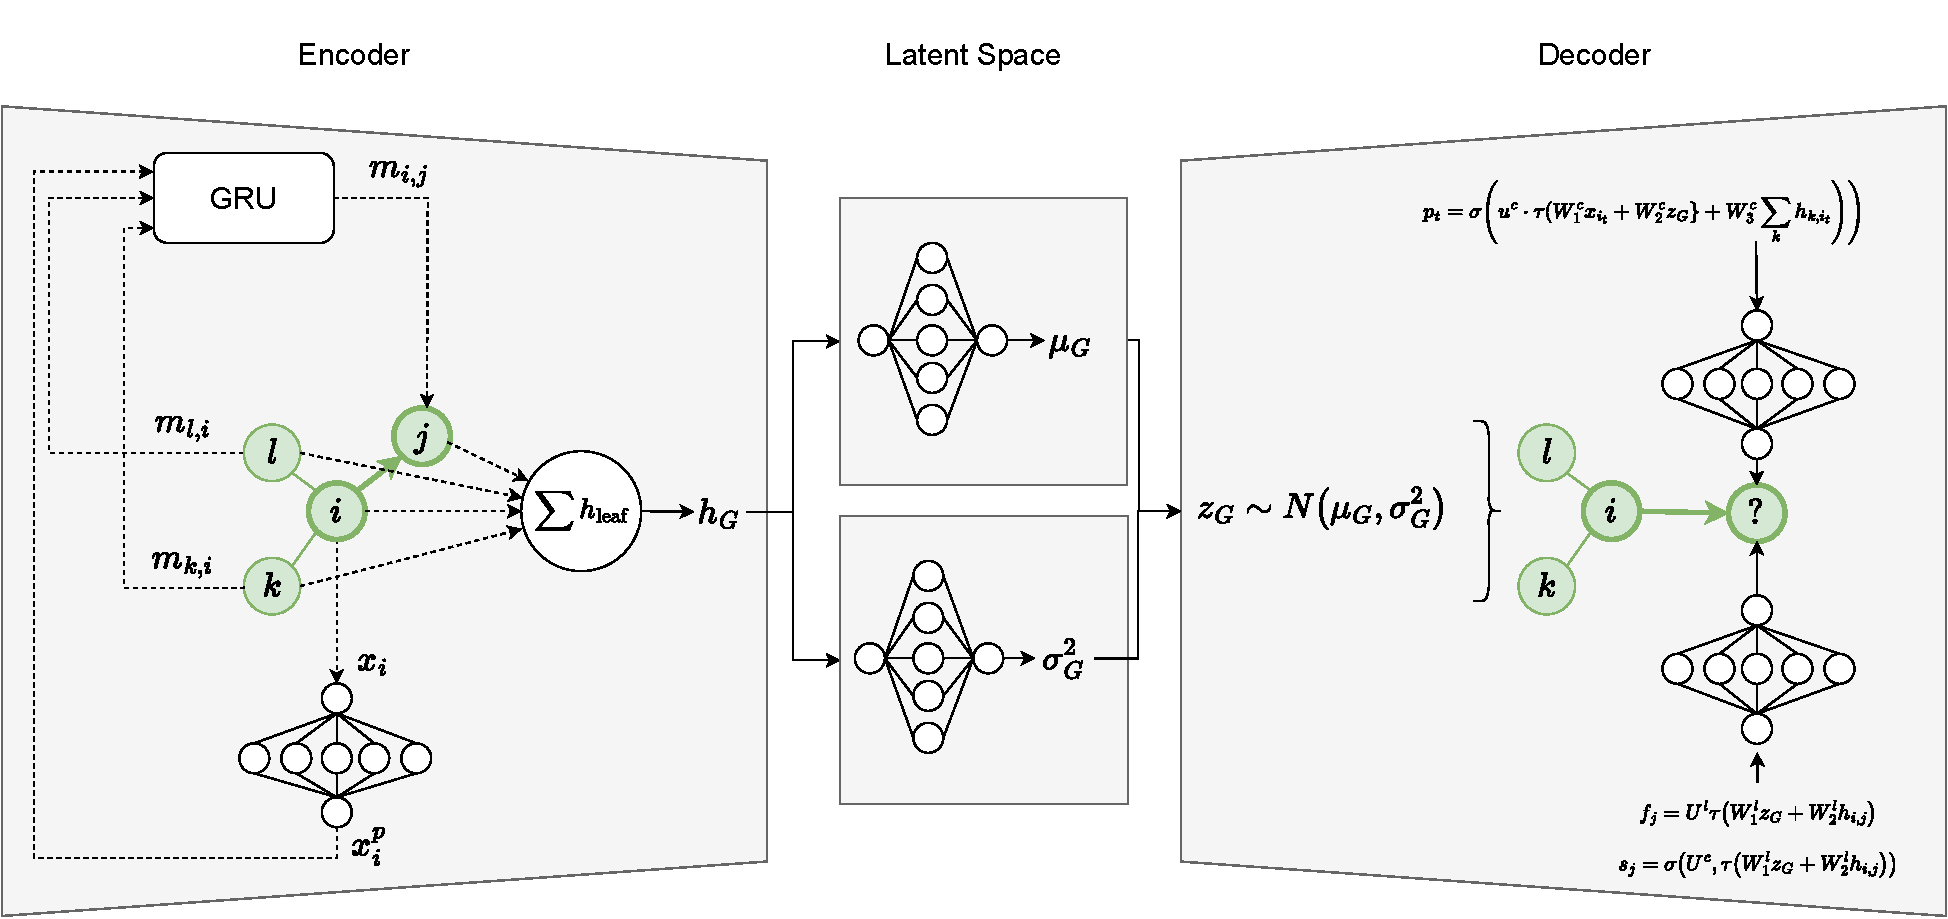
\includegraphics[width=1\textwidth,keepaspectratio]{figures/vae.drawio.pdf}
    \caption{Detailed overview of the proposed VAE design. In the Encoder, the messages of the nodes are updated through a GRU. The features are projected to the hidden state dimension through a learned, linear transformation and the final representation of a graph is obtained by linear transformations and a ReLU activation. Based on this, the mean $\mu_{\mathcal{G}}$ and variance $\sigma^2_{\mathcal{G}}$ are derived by using linear layers. The decoder uses a similar MPNN architecture and expands the constructed graph based on topological prediction and feature regression and categorical prediction for the node type.}
    \label{fig:vae}
\end{figure*}

\subsection{Decoding Robot Designs}

The decoder component of the VAE reconstructs the robot design graph from the continuous latent 
representation $z_G$ through a sequential generation process. Starting from the root node, the 
decoder expands the graph in a depth-first manner by iteratively attaching nodes to the current 
partial design. At each generation step, it performs two tasks: deciding whether to expand the graph and if so, predicting the continuous feature values of the new node.

The decision of expanding the graph is based on message passing within the partial graph. Here, messages are propagated through the same 
GRU architecture used in the encoder. Formally, the probability $p_t$ of expanding the current 
node $i_t$ at time step $t$ is computed as:
\begin{equation}
p_t = \sigma (u^c \cdot \tau (W_1^c x_{i_t} + W_2^c z_{\mathcal{G}} + W_3^c \sum_{k} h_{k,i_t})),
\end{equation}
where $\sigma$ denotes the sigmoid activation, $\tau$ is a ReLU activation, $x_{i_t}$ represents 
the node features, $h_{k,i_t}$ are inward messages from neighboring nodes and $W_1^c$, $W_2^c$, $W_3^c$ are trainable weight matrices, projecting between the latent, hidden and feature spaces.

When a new child node $j$ is created from parent $i$, our approach differs from traditional 
classification-based methods \cite{hu2023glso} by directly regressing the continuous feature values of the node. 
Instead of predicting discrete labels from a vocabulary \cite{zhao2020robogrammar}, the decoder outputs a continuous feature 
vector. In addition, a sigmoid activation is used to determine the node type, distinguishing 
between link and joint nodes in the robot structure. The feature prediction for node $j$ is given by
\begin{align}
f_j &= U^{l} \, \tau \left(W_1^l z_G + W_2^l h_{i,j}\right), \\
s_j &= \sigma \left(U^{c} \, \tau \left(W_1^l z_G + W_2^l h_{i,j}\right)\right),
\end{align}
where $f_j$ denotes the predicted 
feature vector, $s_j$ the predicted node type, $h_{i,j}$ is the message passed from parent $i$ to child $j$ and $W_1^l$, $W_2^l$, $U^l$ and $U^c$ are trainable weights.

The overall decoder loss combines the topological prediction loss, the feature regression loss and the node type classification loss. The topological predictions are trained using binary 
cross-entropy between the predicted probability $p_t$ and the ground truth $\hat{p}_t$. Feature 
regression is optimized using a mean squared error (MSE) loss between predicted features and 
ground truth features. Node type prediction is trained with binary cross-entropy loss based on the 
sigmoid output $s_j$. The total decoder loss is:
\begin{equation}
\mathcal{L}_d(\mathcal{G}) = \sum_{t} \mathcal{L}_c(p_t, \hat{p}_t) + \sum_{j} \Big[ \mathcal{L}_{\text{feat}}(f_j, \hat{f}_j) + \mathcal{L}_{\text{type}}(s_j, \hat{s}_j) \Big],
\end{equation}
where $\mathcal{L}_c$ is the binary cross-entropy for topology decisions, 
$\mathcal{L}_{\text{feat}}$ measures the mean squared error for feature values and 
$\mathcal{L}_{\text{type}}$ is the binary cross-entropy for node type classification. In the forward pass of the VAE this loss and the KL-Divergence from the encoder are added and form the total loss as:
\begin{equation}
    \mathcal{L}(\mathcal{G}) = \mathcal{L}_d(G) + \beta \mathcal{L}_{KL}
\end{equation}
where $\beta$ controls the influence of the KL divergence regularization.

During training, we apply teacher forcing \cite{williams1989learning}: ground truth topology and features are provided at each step to stabilize learning. At inference time, the decoder generates the robot design 
graph autoregressively, relying solely on its own predictions to reconstruct the structure from 
the latent representation $z_G$.

\begin{figure*}[t]
    \centering
    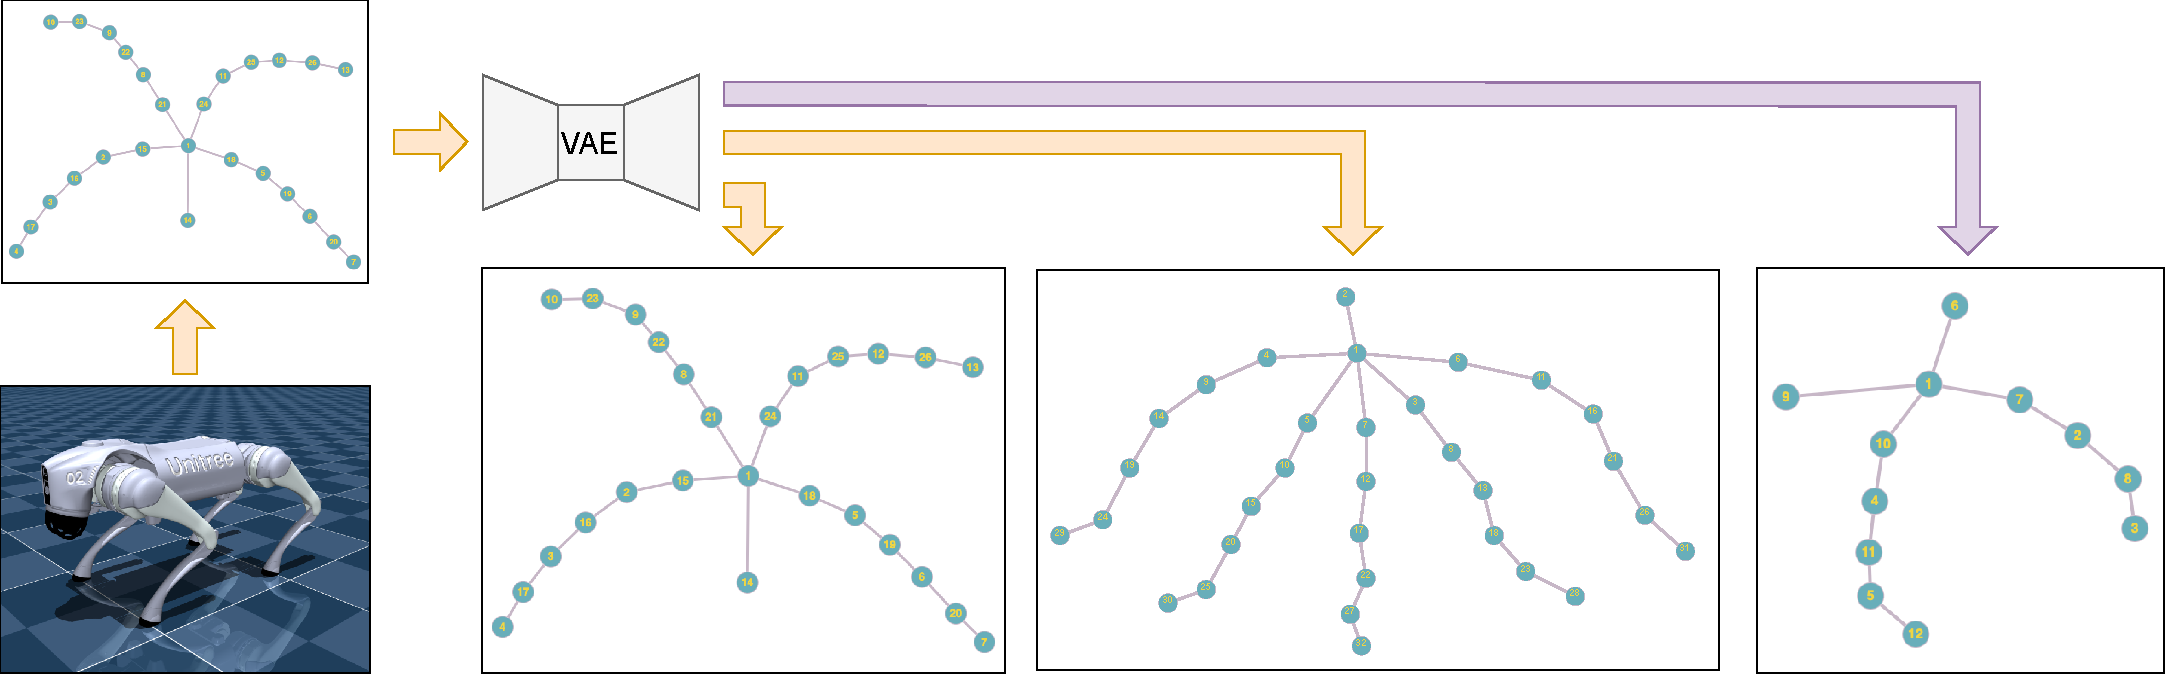
\includegraphics[width=\textwidth]{figures/experimental-results-updated.pdf}
    \caption{Experimental results of encoding and decoding the Unitree Go2 robot for the training datasets consisting of 2 and 4 robot designs. The bottom left and bottom middle graph (orange arrows) show the output of the reconstructed Go2, after the VAE was first trained on two quadrupeds and then on two quadrupeds and humanoids. When trained on two quadrupeds, the reconstruction of the Go2 worked perfectly. However, when adding two humanoids to the training data, the reconstructed graph falsely contains an additional limb. The bottom right graph (purple arrow) shows a new valid graph obtained by sampling from the latent space.}
    \label{fig:experimental_results}
\end{figure*}

\section{Experimental Results}
To test the feasibility and capabilities of our approach, we conducted three experiments, one on synthetic data and two on real robot data. For every dataset, there were mainly two aspects that we investigated: (1) Is the VAE able to encode and decode a new, unseen graph that was not in the training dataset? (2) Does sampling from the learned latent space yield a new, similar graph? 

We chose these two aspects as they effectively capture the requirements for the input-output flow of our model when used for large-scale robot generation: In training, the system receives batches of MuJoCo XML files as input and learns a general latent space representation, which should generalize across embodiments. This is investigated by (1), i.e. encoding and decoding an unseen design. Based on this, the learned latent space can be used to generate novel designs by sampling and decoding, which is investigated by (2). In this case there is no new input to the system. 

To quantify the reconstruction quality in the following experiments, we introduce two metrics: the Reconstruction Accuracy (RA), which is defined as the ratio of correctly reconstructed nodes to the total number of nodes in the output graph, and the Feature Reconstruction Error (FRE), which is defined as the MSE between predicted and ground-truth feature values.

For the synthetic examples, we abstracted from a specific robot in order to directly use adjacency matrices of undirected, acyclic graphs. We started with a small example dataset of 20 random graphs consisting of 15 nodes each and five-dimensional feature vectors with random values between 0 and 1. 

For both questions, our VAE yielded promising results on the synthetic data. It was able to reconstruct the same structure, i.e. the nodes and predicted the continuous feature values of an unseen graph with minimal deviation from the ground truth values. Also sampling from the learned latent space gave us a valid graph structure. Training plots for these experiments can be found in appendix \ref{synth_training_plot}.

Based on this, we continued with real robot data from the MujoCo Menagerie \cite{menagerie2022github}, a collection of high-quality models of real robots. We focused on robots that were able to perform locomotion tasks, as the first use case of our system will be generating robots for downstream cross-embodiment locomotion policy training \cite{bohlinger2024one, ai2025towards}. In total, we used 34-dimensional feature vectors containing the physical attributes of the model, which are listed in appendix \ref{physical-parameters}.

In the first step, we tested the validity of our preprocessing by overfitting the VAE on one robot design. Since the RA was $100\%$ and the FRE was approximately zero, we expanded our training dataset to first two quadrupeds and afterwards added two humanoids (see appendix \ref{robots_training_data}). After training, we tested the VAE on encoding and decoding the Unitree Go2 robot, which was not in the training data. The VAE solely trained on quadrupeds was able to reconstruct the Go2 perfectly with a RA of $100\%$. However, the VAE trained on both quadrupeds and humanoids had a RA of $81\%$ and showed a similar but incorrect structure with one additional limb. After investigation we conclude that the MPNN falsely predicts one additional node expansion from the root node. We assume that the MPNN learned that a node connecting to the root is always expanded to a full limb which explains the mismatch in comparision to the input graph. 

The continuous feature reconstruction worked well in both cases with a FRE of approximately $10^{-3}$ (the additional fifth limb was excluded from the computation as there are no ground-truth feature values for it). We hypothesized that a larger and more diverse dataset would improve the reconstruction performance of the VAE. The specific robots that were used for training can be found in appendix \ref{robots_training_data}.

Additionally, we sampled a random vector from the latent space and ran the vector through the learned decoder. This yielded a valid graph structure but it is arguable whether this will result in a usable MuJoCo design after applying postprocessing. The results of these experiments are summarized in \cref{fig:experimental_results}. The training plots can be found in appendix \ref{4_training_plots}.

\begin{figure*}[t]
    \centering
    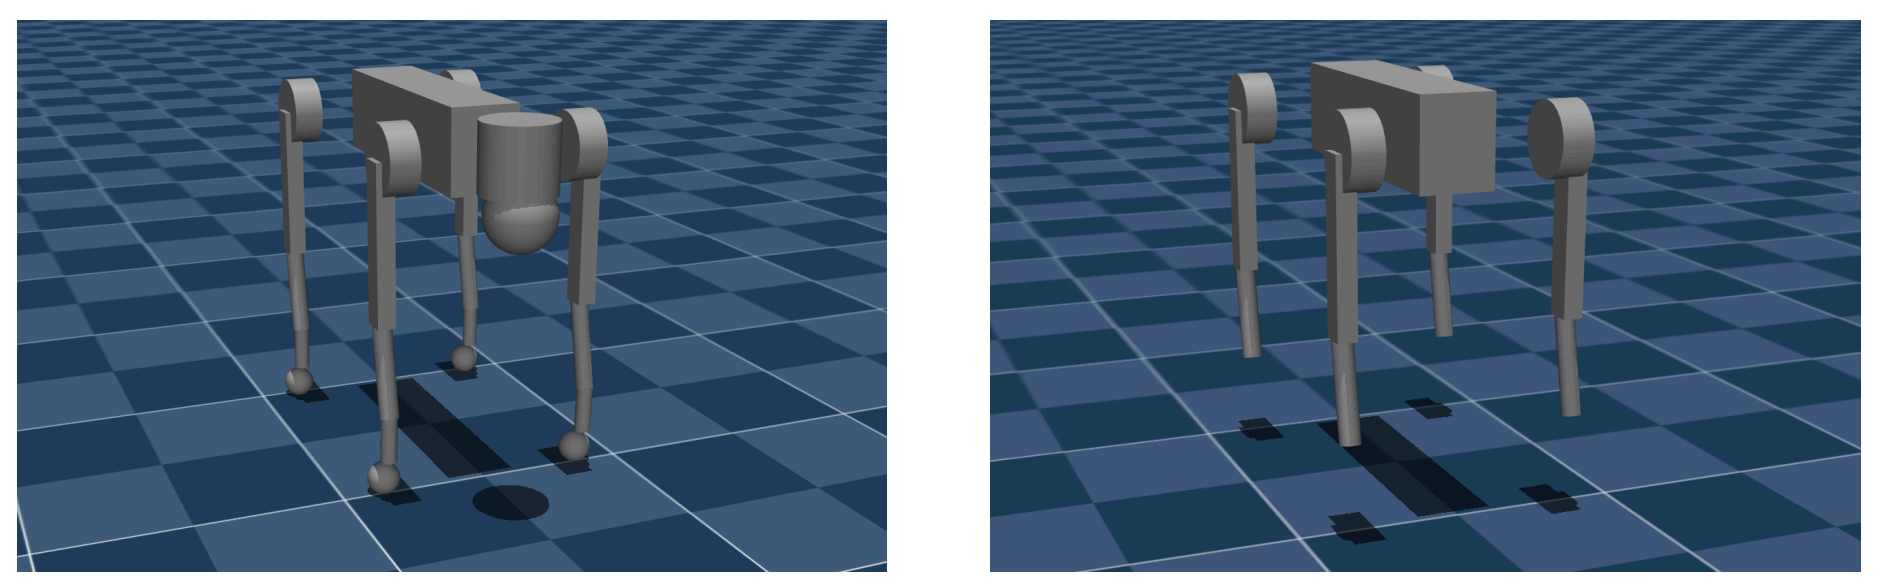
\includegraphics[width=\textwidth]{figures/go2_recon_2.png}
    \caption{Comparison between the original Unitree Go2 (left) and the reconstructed Go2 obtained from our decoder and the postprocessing pipeline (right). The reconstruction captures the general four-limbed morphology of the robot, while missing certain parts such as the feet and head as only one geom is considered per body part.}
    \label{fig:recon}
\end{figure*}

To further evaluate our approach, we passed the reconstructed Unitree Go2 through our postprocessing pipeline and visualized the result in \cref{fig:recon}, where it is shown side by side with the original Unitree Go2. For clarity, we only show the reconstructed version of the robot that has four limbs, as this allows a direct comparison to the reference robot. The visualization shows that our reconstruction captures the general form of the robot, while some parts such as the feet and head are missing. This happens because the current postprocessing only considers a single geom per body part. Since the main physical properties, such as mass and inertia, are defined directly in the links, these missing geoms do not severely affect the viability of the reconstructed robot, as they are primarily used for visualization and collision detection.


Based on this, we expanded the training dataset to 17 robots of the MuJoCo Menagerie. As hypothesized, increasing the diversity of the training data improved the structural reconstruction as the encoding and decoding of the Unitree Go2 yielded a reconstruction accuracy of $100\%$. However, the FRE remained relatively high. This was anticipated as the FRE directly corresponds to the MSE term in the training loss, which had not converged after 1500 epochs with normalized features (see in the training plots in appendix \ref{25_training_plots}). Training for additional epochs would likely reduce this loss further, but due to time constraints we were not able to compute longer runs.

\section{Discussion and Future Work}
Our current work demonstrates the feasibility of using a VAE framework with an MPNN for large-scale robot generation. However, several aspects remain open for further development and evaluation. In the following, we highlight key directions.

\subsection{Postprocessing}
A critical component, which needs to be expanded is the postprocessing pipeline that converts the decoded graph representation back into a valid MuJoCo XML file. While our current postprocessing returns the basic XML structure, the  additional geometric properties present further challenges. 

In MuJoCo the geometric properties of a body describe its appearance and their dimensionality varies depending on the type. Currently, we only take the default type into account which limits the usage of the reconstructed model. Adapting this requires additional changes in the postprocessing to ensure a valid reconstruction of the learned geometric properties. 

Additionally, the decoded continuous features have to be mapped to valid physical parameters, ensuring constraints such as non-negative masses valid joint limits and unit quaternions. We assume that by providing valid physical attributes in the training data, the VAE only learns feasible attributes. This assumption may fail in edge cases such as joint ranges outside the ones available in MuJoCo, negative masses or non-normalized quaternions. These cases can be addressed by simple mapping rules to constrain the output to the ranges available in MuJoCo, e.g. by clipping negative masses to zero and normalizing quaternion outputs to enforce unit length. 

These steps are important not only for the visualization of the generated robots, but also for validating whether our generated robots are structurally and physically plausible for simulation and downstream tasks.

\subsection{Statistical View of Robot Generation}
The learned latent space does not only enable us to generate many different robots through sampling, but offers us the opportunity to analyze robot populations from a statistical perspective. 

By treating the latent distribution as a representation of the robot design space, one could quantify similarity and diversity among embodiments. In future work we plan to use an entropy-based encoding strategy similar to those employed in Task-Agnostic Morphology Evolution \cite{hejna2021task} to characterize differences between robot morphologies. This approach may provide a statistical way to understand the learned design space.

\subsection{Robot Design Validation}
An additional important next step will be to test whether the reconstructed robots are physically and functionally feasible. For this, we plan to use a trained locomotion policy on the original Unitree Go2 and apply it to the reconstructed Go2 produced by our decoder. If the policy transfers successfully, it would indicate that the generated robot designs are not only valid in terms of graph structure and features but also usable in downstream tasks.

% In the unusual situation where you want a paper to appear in the
% references without citing it in the main text, use \nocite
\nocite{langley00}

\bibliography{lascroge}
\bibliographystyle{icml2025}


%%%%%%%%%%%%%%%%%%%%%%%%%%%%%%%%%%%%%%%%%%%%%%%%%%%%%%%%%%%%%%%%%%%%%%%%%%%%%%%
%%%%%%%%%%%%%%%%%%%%%%%%%%%%%%%%%%%%%%%%%%%%%%%%%%%%%%%%%%%%%%%%%%%%%%%%%%%%%%%
% APPENDIX
%%%%%%%%%%%%%%%%%%%%%%%%%%%%%%%%%%%%%%%%%%%%%%%%%%%%%%%%%%%%%%%%%%%%%%%%%%%%%%%
%%%%%%%%%%%%%%%%%%%%%%%%%%%%%%%%%%%%%%%%%%%%%%%%%%%%%%%%%%%%%%%%%%%%%%%%%%%%%%%
\newpage
\appendix
\onecolumn

\section{Robots included in Training Datasets for experiments} \label{robots_training_data}
The training dataset for the experiment with 2 robots consisted of: \textit{Unitree Go1}, \textit{Unitree A1}.

The training dataset for the experiment with 4 robots consisted of: \textit{Unitree Go1}, \textit{Unitree G1}, \textit{Unitree A1}, \textit{Unitree H1}.

The training dataset for the experiment with 17 robots consisted of: \textit{Agility Piper}, \textit{Agility Cassie}, \textit{Berkeley Humanoid}, \textit{Booster T1}, \textit{Boston Dynamics Spot}, \textit{Fourier N1}, \textit{Google Barkour V0}, \textit{Google Barkour VB}, \textit{PAL Talos}, \textit{PAL Tiago}, \textit{PAL Tiago Dual}, \textit{Unitree A1}, \textit{Unitree G1}, \textit{Unitree Go1}, \textit{Unitree Go2}, \textit{Unitree H1} and \textit{Unitree Z1}.

\section{Training Plots for Experiments on Synthetic Data} \label{synth_training_plot}

\begin{figure}[!htbp]
\centering

\includegraphics[width=0.40\textwidth,keepaspectratio]{figures/training_plots_synthetic/pred_loss.png}
\hfill

\includegraphics[width=0.40\textwidth,keepaspectratio]{figures/training_plots_synthetic/stop_loss.png}
\caption{Training Plots for Experiments on Synthetic Data. For better visibility due to different orders of loss magnitudes, the prediction loss is clipped at 0.02 and the stop loss at 0.001}
\end{figure}


\section{Training Plots for Experiments on 4 Robots of MuJoCo Menagerie} \label{4_training_plots}

\begin{figure}[!htbp]
\centering

\includegraphics[width=0.40\textwidth,keepaspectratio]{figures/training_plots_menagerie_6/pred_loss.png}
\hfill

\includegraphics[width=0.40\textwidth,keepaspectratio]{figures/training_plots_menagerie_6/stop_loss.png}
\caption{Training Plots for Experiments on 4 Robots of MuJoCo Menagerie. For better visibility due to different orders of loss magnitudes, the plot starts at epoch 500 and is clipped at 0.1 for the prediction loss and at 0.001 for the stop loss.}
\end{figure}
\newpage
\section{Training Plots for Experiments on 17 Robots of MuJoCo Menagerie} \label{25_training_plots}

\begin{figure}[!htbp]
\centering
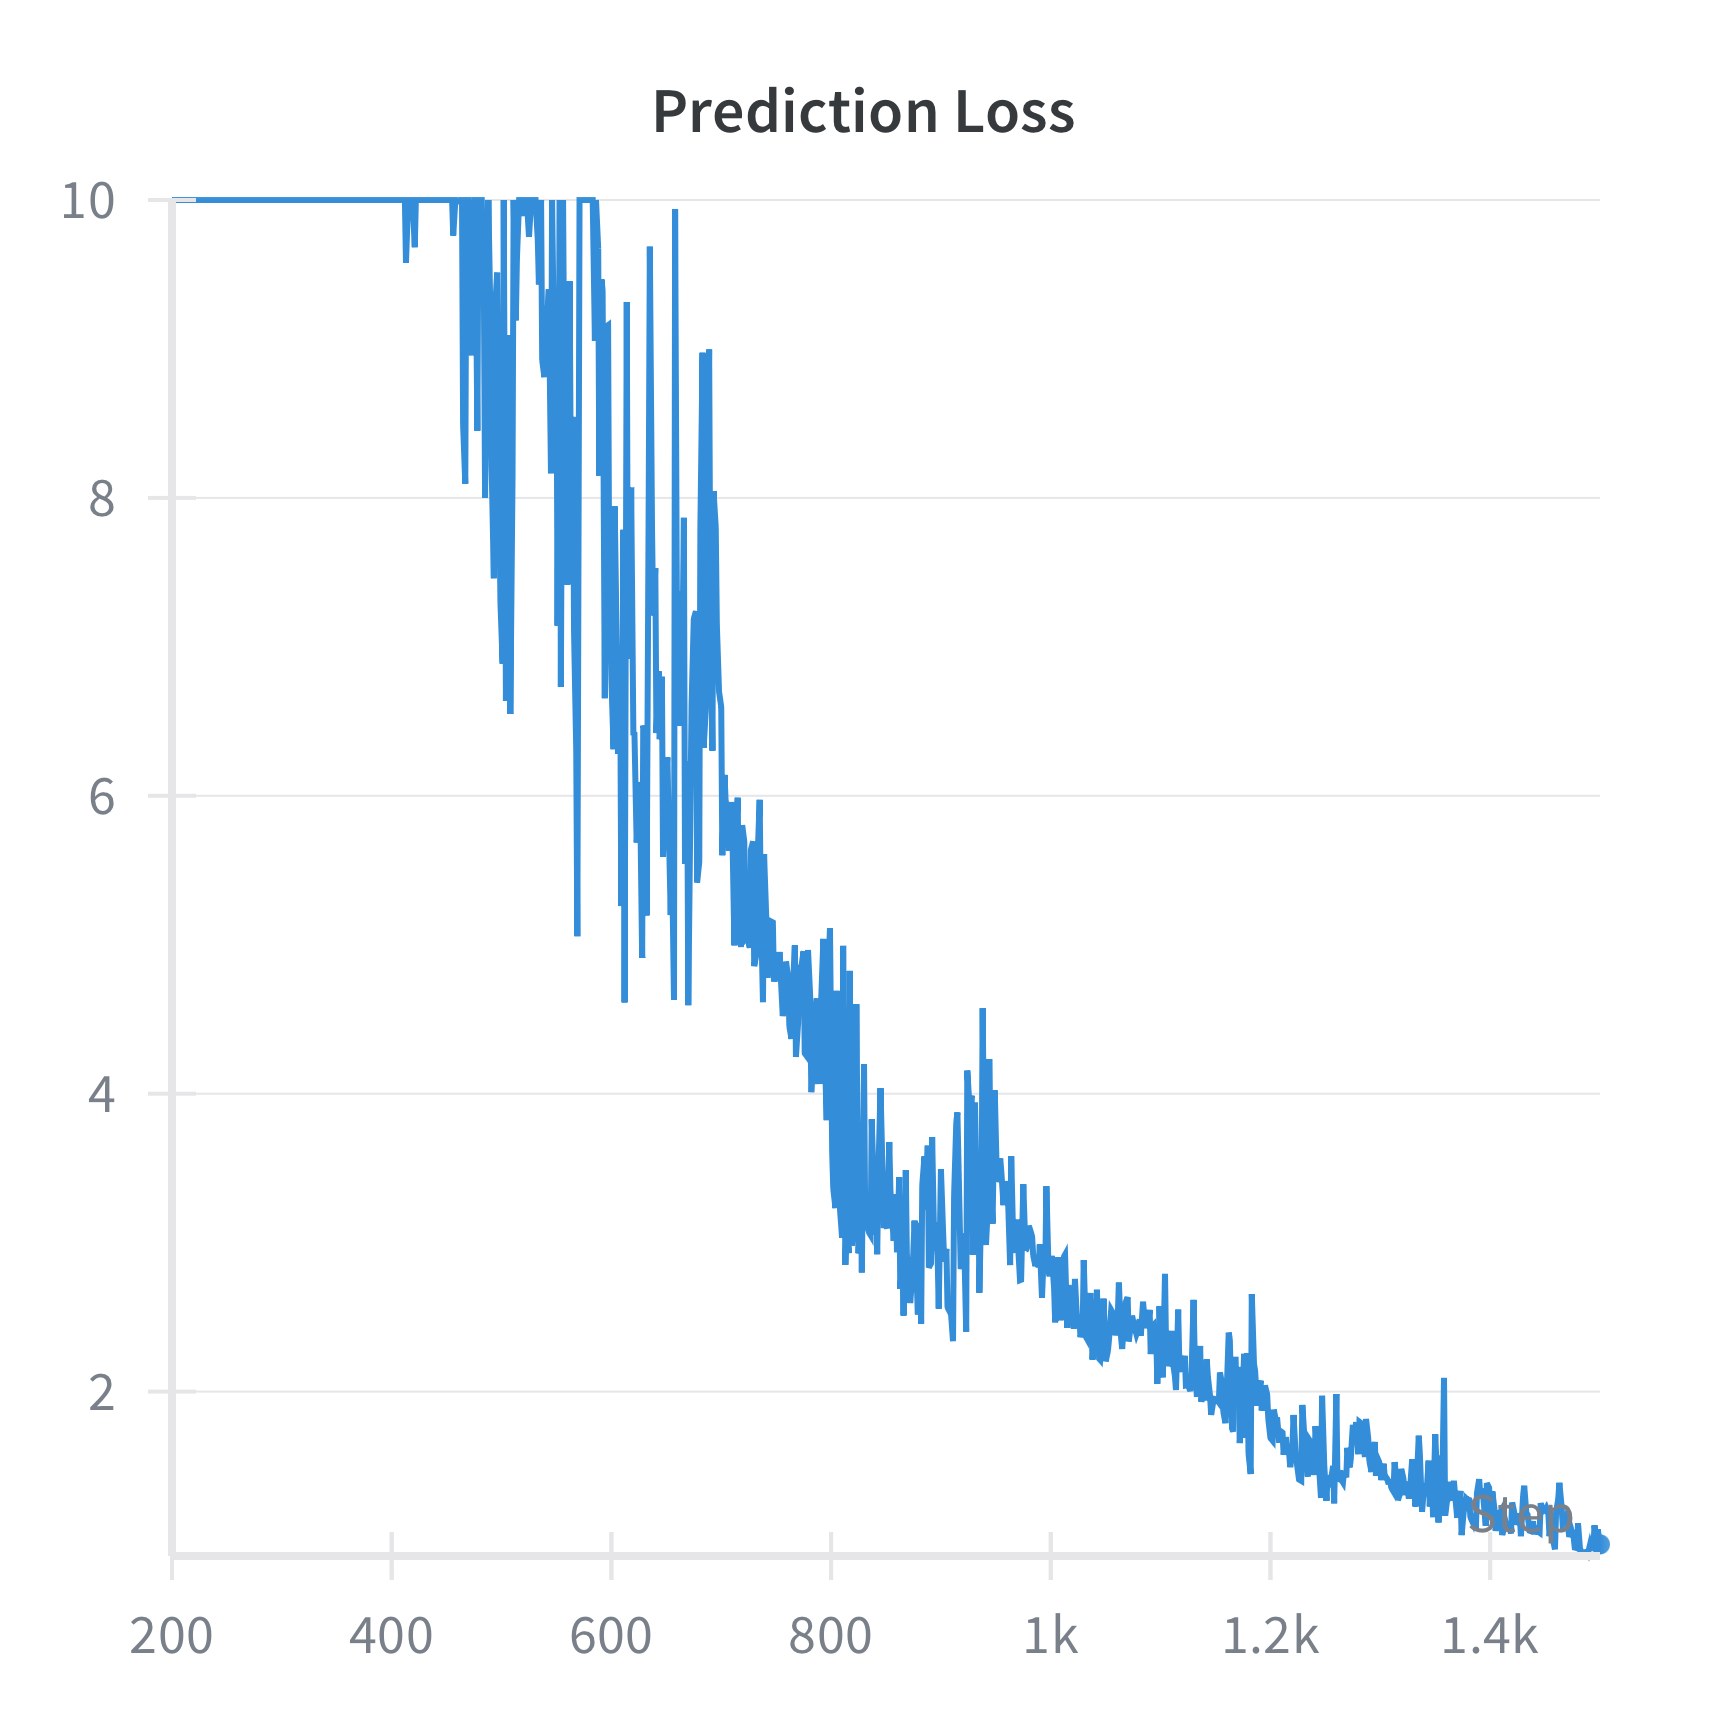
\includegraphics[width=0.40\textwidth,keepaspectratio]{figures/training_plots_menagerie_25/pred_loss.png}
\hfill
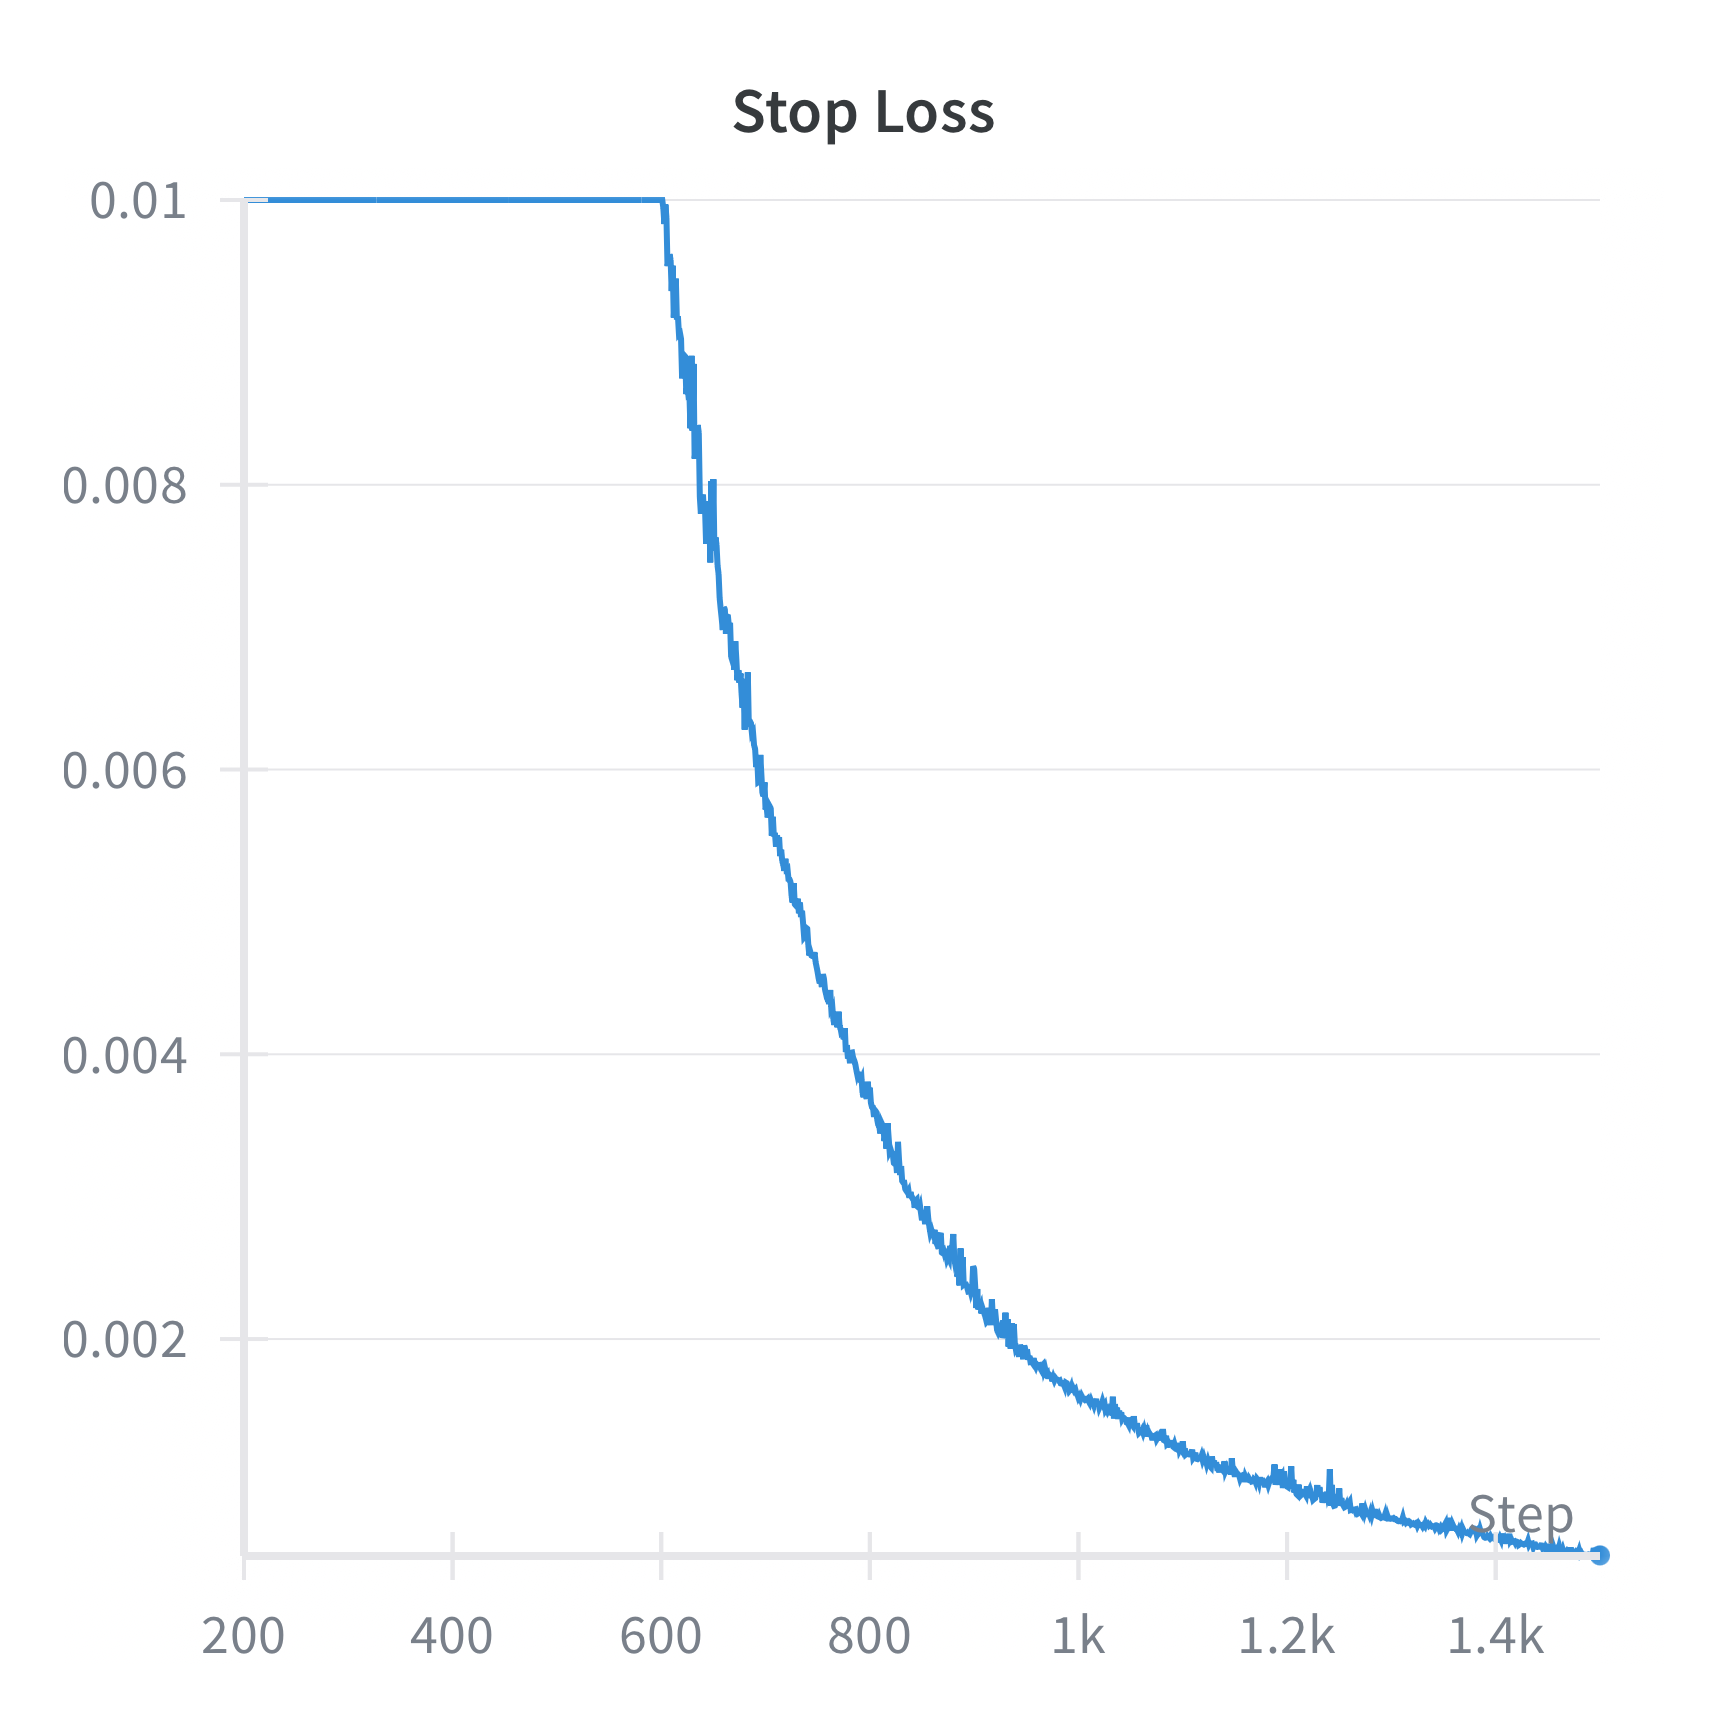
\includegraphics[width=0.40\textwidth,keepaspectratio]{figures/training_plots_menagerie_25/stop_loss.png}
\caption{Training Plots for Experiments on 17 Robots of MuJoCo Menagerie. For better visibility due to different orders of loss magnitudes, the plot starts at epoch 200 and is clipped at 10 for the prediction loss and at 0.01 for the stop loss.}
\end{figure}


\section{Physical Parameters used during Training on Robots of MuJoCo Menagerie}\label{physical-parameters}
\begin{table}[h]
\centering
\caption{Features of the MuJoCo models used during training}
\label{tab:features}
\begin{tabular}{llll}
\toprule
\textbf{Feature} & \textbf{Node type} & \textbf{Description} & \textbf{Value Range} \\
\midrule
range      & Joint & Allowed motion limits for the joint     & $[\theta_{\min}, \theta_{\max}]$ (radians) \\
stiffness  & Joint & Joint stiffness (spring constant)       & $\geq 0$ \\
axis       & Joint & Axis of rotation / translation          & unit vector in $\mathbb{R}^3$ \\
pos        & Joint & Anchor position of the joint            & world/local coordinates \\
armature  & Joint & Added rotational inertia for joint DoF & $\geq 0$ (kg$\cdot$m$^2$) \\
damping       & Joint & Viscous damping coefficient resisting motion & $\geq 0$ \\
frictionloss        & Joint & Static frictional torque/force before motion occurs & $\geq 0$ \\
\midrule
pos        & Body  & Body or geom position in frame          & world/local coordinates \\
mass       & Body  & Mass of the body                       & $\geq 0$ \\
inertia    & Body  & Inertia matrix components              & $\geq 0$ \\
quat       & Body  & Orientation of body or geom            & unit quaternion \\
subtreemass& Body  & Mass of body + descendants             & $\geq 0$ \\
ipos       & Body  & Joint anchor position in body frame    & world/local coordinates \\
iquat      & Body  & Joint orientation in body frame        & unit quaternion \\
size       & Body  & Geometric size (radius, length, etc.)  & $\geq 0$ \\
\bottomrule
\end{tabular}
\end{table}

%%%%%%%%%%%%%%%%%%%%%%%%%%%%%%%%%%%%%%%%%%%%%%%%%%%%%%%%%%%%%%%%%%%%%%%%%%%%%%%
%%%%%%%%%%%%%%%%%%%%%%%%%%%%%%%%%%%%%%%%%%%%%%%%%%%%%%%%%%%%%%%%%%%%%%%%%%%%%%%


\end{document}

